\section{Several vertices at once}
%<-------------------------------------------------------------------------->
\tkzcname{Vertices} places a list of vertices on a line or on a simple
geometric figure: triangle, square or circle.

\begin{NewMacroBox}{Vertices}{\oarg{local options}\var{form}\var{list of vertices}}
\begin{tabular}{llc}
\toprule
First argument   &  & Definition            \\
\midrule
\TAline{line}   {} {vertices on a line; the option \tkzname{dir} gives the direction}
\TAline{tr1}    {} {first form of triangle}
\TAline{tr2}    {} {second form of triangle}
\TAline{tr3}    {} {third form of triangle}
\TAline{tr4}    {} {fourth form of triangle}
\TAline{square} {} {four vertices on a square}
\TAline{circle} {} {vertices on a circle (regular polygon)}
\bottomrule
\end{tabular}

\medskip
\emph{The second argument is a list of names of vertices.}

\medskip
\begin{tabular}{llc}
\toprule
Options   & Default  &      Definition  \\
\midrule
\TOline{dir}       {\textbackslash EA}{direction of a line}
\TOline{unit}      {\textbackslash GraphUnit}{side, or radius of the circle}
\TOline{rotation}  {0}{\tkzname{circle}: angle of the first vertex}
\TOline{clockwise} {false}{\tkzname{circle}: the vertices turn clockwise}
\bottomrule
\end{tabular}

\medskip
\emph{The other options are those of \tkzcname{Vertex}; they apply to every
vertex. For a line, the possible directions are \tkzcname{EA},
\tkzcname{WE}, \tkzcname{NO}, \tkzcname{SO}, \tkzcname{NOEA},
\tkzcname{NOWE}, \tkzcname{SOEA} and \tkzcname{SOWE}.}
\end{NewMacroBox}

\subsection{A line from a given point}
\begin{tkzexample}[latex=7cm,small]
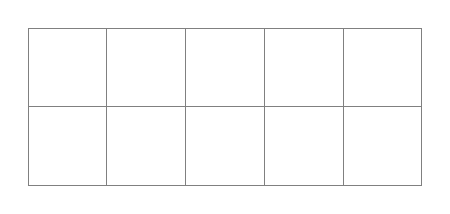
\begin{tikzpicture}
  \SetGraphUnit{2}
  \draw[help lines] (0,0) grid (5,2);
  \Vertices[x=1,y=2]{line}{A,B,C}
\end{tikzpicture}
\end{tkzexample}

\subsection{A line from an existing node}
\begin{tkzexample}[latex=7cm,small]
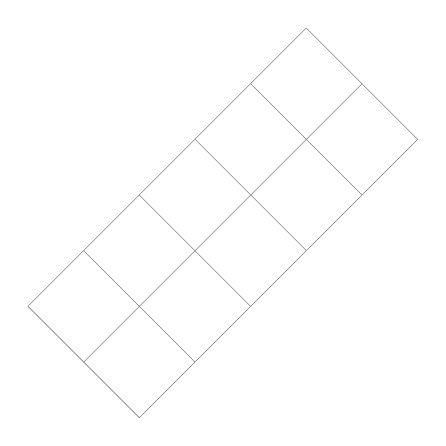
\begin{tikzpicture}[rotate=45]
  \SetGraphUnit{2}
  \draw[help lines] (0,0) grid (5,2);
  \coordinate (A) at (1,1);
  \Vertices[Node]{line}{A,B,C}
\end{tikzpicture}
\end{tkzexample}

\subsection{Lines with a direction}
\begin{tkzexample}[latex=7cm,small]
\begin{tikzpicture}
  \GraphInit[vstyle=Art]
  \Vertices[dir=\NOEA]{line}{A,B,C,D}
  \Vertices[dir=\NOWE]{line}{A,E,F,G}
\end{tikzpicture}
\end{tkzexample}

\subsection{Triangles}
The triangles are right isosceles triangles. Here are the forms
\tkzname{tr1}, \tkzname{tr2}, \tkzname{tr3} and \tkzname{tr4}.

\begin{tkzexample}[latex=8cm,small]
\begin{tikzpicture}\SetGraphUnit{2}
  \Vertices{tr1}{A,B,C}\Edges(A,B,C,A)
\end{tikzpicture}\hspace*{1cm}
\begin{tikzpicture}\SetGraphUnit{2}
  \Vertices{tr2}{A,B,C}\Edges(A,B,C,A)
\end{tikzpicture}
\end{tkzexample}

\begin{tkzexample}[latex=8cm,small]
\begin{tikzpicture}\SetGraphUnit{2}
  \Vertices{tr3}{A,B,C}\Edges(A,B,C,A)
\end{tikzpicture}\hspace*{1cm}
\begin{tikzpicture}\SetGraphUnit{2}
  \Vertices{tr4}{A,B,C}\Edges(A,B,C,A)
\end{tikzpicture}
\end{tkzexample}

\subsection{A square}
The center of the square is obtained with an intersection (see the
\tkzname{pgfmanual}).

\begin{tkzexample}[latex=7cm,small]
\begin{tikzpicture}
  \SetGraphUnit{3}
  \GraphInit[vstyle=Shade]
  \Vertices{square}{A,B,C,D}
  \coordinate (E) at (intersection of A--C and B--D);
  \Vertex[Node]{E}
\end{tikzpicture}
\end{tkzexample}

\newpage
\subsection{A circle}
By default the first vertex is at the angle $0$ and the vertices turn
counterclockwise.

\begin{tkzexample}[latex=7cm,small]
\begin{tikzpicture}
  \SetGraphUnit{2}
  \Vertices{circle}{A,B,C,D,E}
\end{tikzpicture}
\end{tkzexample}

\subsubsection{Options \tkzname{rotation} and \tkzname{clockwise}}
\tkzname{rotation} gives the angle of the first vertex; with
\tkzname{clockwise}, the vertices turn clockwise.

\begin{tkzexample}[latex=7cm,small]
\begin{tikzpicture}
  \SetGraphUnit{2}
  \Vertices[rotation=90,clockwise]{circle}{A,B,C,D,E}
  \Edges(A,B,C,D,E,A)
\end{tikzpicture}
\end{tkzexample}

\subsubsection{A circle and outside labels}
With an outside label, \tkzname{Lpos} is added to the angle of each vertex:
the labels follow the rotation of the figure.

\begin{tkzexample}[latex=7cm,small]
\begin{tikzpicture}
  \SetGraphUnit{2}
  \GraphInit[vstyle=Classic]
  \Vertices{circle}{A,B,C,D,E,F}
\end{tikzpicture}
\end{tkzexample}

\begin{tkzexample}[latex=7cm,small]
\begin{tikzpicture}
  \GraphInit[vstyle=Classic]
  \Vertices[unit=2,rotation=90]{circle}{A,B,C,D,E,F}
\end{tikzpicture}
\end{tkzexample}

\subsubsection{A circle and a shortcut}
\begin{tkzexample}[latex=7cm,small]
\begin{tikzpicture}[scale=.5]
  \SetGraphUnit{4}
  \GraphInit[vstyle=Classic]
  \Vertices[rotation=45]{circle}{C,E,A,B}
  \NOEA[unit=2.828](E){D}
  \Edges(A,B,E,D,C,E,A,C,B)
\end{tikzpicture}
\end{tkzexample}

\endinput
